\section{Experiments} \label{sec:experiment}
In this section, we measure the overall performance of the optimized 
HLS based BFS accelerator on Alpha Data ADM-PCIE-7v3 using a set of 
representative graphs. Then we compare the resulting accelerator to 
both a baseline design which has best-effort HLS optimization applied to 
native BFS code and existing FPGA based BFS acceleration work. Then we evaluate 
the major design optimization methods including pipelining, redundancy removal,  
caching and data path duplication proposed in this work. 

\subsection{Experiment Setup}
The graph benchmark used in this work includes three real-world graphs and 
two synthetic graphs generated using R-MAT model \cite{chakrabarti2004rmat} 
as listed in Table \ref{tab:graph}. The real-world graphs are from social network \cite{yang2012defining, 
leskovec2009community, takac2012data} while the R-MAT graphs are generated 
using the Graph 500 benchmark parameters ($A=0.59, B=0.19, C=0.19$). To make the 
presentation easier, the five benchmark graphs are shorted as Youtube, 
LJ, Pokec, R-MAT\uppercase\expandafter{\romannumeral1}, 
R-MAT\uppercase\expandafter{\romannumeral2} respectively. We refer 
to an R-MAT graph with scale $S$ ($2^{S}$ nodes) and edge factor $E$ ($E\times 2^{S}$). 
In order to avoid trivial search, we only choose vertices from the largest 
connected component as the BFS starting point.

\begin{table}
    \centering
  \caption{Graph Benchmark}
  \label{tab:graph}
  \begin{tabular}{cccc}
    \toprule
      Name & \# of vertex & \# of edge & Type \\
    \midrule
      Youtube \cite{yang2012defining} & 1157828 & 2987624 & Undirectional \\
      LJ \cite{leskovec2009community} & 4847571 & 68993773 & Directional \\
      Pokec \cite{takac2012data} & 1632804 & 30622564 & Directional \\
      R-MAT\uppercase\expandafter{\romannumeral1} & 524288 & 16777216 & Directional \\
      R-MAT\uppercase\expandafter{\romannumeral2} & 2097152 & 67108864 & Directional \\
  \bottomrule
\end{tabular}
\end{table}

\subsection{Performance comparison}
We use the million traverse per second (MTEPS) as 
the performance metric. The performance of the proposed BFS 
accelerator on the graph benchmark is 
presented in Table \ref{tab:performance-summary}. 
It gets up to 82.16 MTEPS on the R-MAT\uppercase\expandafter{\romannumeral1} graph and achieves 
38.83 MTEPS on average. When compared to a baseline HLS based 
BFS accelerator, the proposed design shows 24.7X to 77.5X performance 
speedup on the five benchmark graphs. Note that the baseline HLS design 
refers to a native C/C++ based BFS implementation 
with best effort HLS pragma optimization but no modification of the source code.
With the comparison, it is clear that straightforward HLS optimizations 
are far from sufficient and dedicated high level optimizations are critical to 
the performance of the resulting BFS accelerator.
\begin{table}
    \centering
  \caption{Performance summary}
  \label{tab:performance-summary}
  \begin{tabular}{cccccc}
    \toprule
      Benchmark & Youtube & LJ & Pokec & RMAT\uppercase\expandafter{\romannumeral1} & RMAT\uppercase\expandafter{\romannumeral2} \\
    \midrule
      MTEPS & 14.35 & 28.05 & 36.94 & 82.16 & 32.67 \\
      Speedup & 77.50 & 36.82 & 38.83 & 62.18 & 24.70 \\
  \bottomrule
\end{tabular}
\end{table}

On top of the comparison to the baseline HLS design, we also compare 
this work to a set of existing BFS accelerators on FPGAs. As the platforms 
and graph benchmark used in these work are mostly different, it is 
difficult to make a fair end-to-end comparison. Hereby, we add
MTEPS per unit bandwidth (MTEPSPB) as an additional performance metric showing the 
potential of the BFS accelerators on different hardware platforms. 
A rough comparison result is listed in Table \ref{tab:compare}. It can be found that the HLS 
based BFS accelerator proposed in this work achieves around 35\% of the 
performance in \cite{zhang2017boosting}. Nevertheless, the memory bandwidth 
is much lower compared to that in \cite{zhang2017boosting} and the per bandwidth 
MTEPS in this work outperforms especially on the R-MAT graphs. Compared to the 
general graph processing framework based BFS accelerator in \cite{dai2016fpgp} and 
\cite{nurvitadhi2014graphgen}, this work shows competitive per bandwidth MTEPS on either 
the R-MAT graph or the graph benchmark. When compared to design on high-end 
FPGA computing system, the performance is still much lower while the per bandwidth 
performance is around 25\% of the highly optimized handcraft design and 
the HLS based design gains the software-like features.

\begin{table}
  \caption{FPGA based BFS accelerator comparison}
  \label{tab:compare}
    \setlength{\tabcolsep}{4pt} % Default value: 6pt
    %\renewcommand{\arraystretch}{1.5} % Default value: 1
  \begin{tabular}{cccccc}
    \toprule
      Work & Platform & Graph & MTEPS & BW(GB/s) & MTEPSPB \\
    \midrule
      \cite{betkaoui2012reconfigurable} & Convey HC-2 & R-MAT & 1600 & 80  & 20 \\
      \cite{attia2014cygraph} & Convey HC-2 & R-MAT    & 1900 & 80  & 24.4 \\
      \cite{zhang2017boosting} & Micro-AC510       & R-MAT  & 166.2  & 60  & 2.8 \\
      \cite{nurvitadhi2014graphgen} & VC707 Kit & Twitter & 148.6 & 6.4 & 9.9 \\
      \cite{dai2016fpgp}  & VC707 Kit & Twitter & 12  & 6.4 & 1.9 \\
      this work & ADM-PCIe-7v3 & R-MAT & 57.41 & 10.8 & 5.3 \\
      this work & ADM-PCIE-7v3 & Graph in Table \ref{tab:graph} & 38.8 & 10.8 & 3.6 \\
  \bottomrule
\end{tabular}
\end{table}

\subsection{Runtime distribution}
According to the experiments, we find that more pipeline stages are typically beneficial to 
the final performance. Particularly, we observe that the resulting BFS accelerator 
performance has significant improvement when the number of pipeline stages 
jumps from 1 to 2 and from 5 to 6. Thus we try to keep the critical pipeline stages 
and further construct new pipeline configurations i.e. c8 and c9. 
The performance, however, is not improved as expected. The comparison also indicates 
that the internal pipeline stages are also important to the 
overall BFS accelerator performance. It is just that they are dependent 
and any one of the sub function that fails to be pipelined will 
stall the overall pipeline and affect the final performance. 
According to the performance and resource consumption experiments, we find that 
c6 achieves near optimal performance with reasonable hardware resource overhead.
Therefore, it is taken as the optimized pipelining setup in the following experiments.

\begin{table}
  \caption{FPGA resource consumption with different pipelining configurations}
  \label{tab:hash-resource}
  %\setlength{\tabcolsep}{4pt} % Default value: 6pt
  %\renewcommand{\arraystretch}{1.5} % Default value: 1
    \centering
  \begin{tabular}{ccccccc}
    \toprule
      Config. & FF & \% & LUT & \% & RAMB18K & \% \\
    \midrule
      c1 & 3581 & $\sim$0 & 4289 & $\sim$0 & 8  & $\sim$0 \\
      c2 & 4121 & $\sim$0 & 5416 & $\sim$1 & 10 & $\sim$0 \\
      c3 & 4208 & $\sim$0 & 5746 & $\sim$1 & 10 & $\sim$0 \\
      c4 & 4494 & $\sim$0 & 6675 & $\sim$1 & 10 & $\sim$0 \\
      c5 & 4551 & $\sim$0 & 7022 & $\sim$1 & 10 & $\sim$0 \\
      c6 & 5546 & $\sim$0 & 8126 & $\sim$1 & 12 & $\sim$0 \\
      c7 & 5853 & $\sim$0 & 8154 & $\sim$1 & 12 & $\sim$0 \\
      c8 & 5113 & $\sim$0 & 7152 & $\sim$1 & 12 & $\sim$0 \\
      c9 & 5408 & $\sim$0 & 7843 & $\sim$1 & 12 & $\sim$0 \\
  \bottomrule
\end{tabular}
\end{table}

\subsubsection{Replication factor}
\subsubsection{Data reorganization}
We explore the correlation between prefetch buffer size and  
buffer hit rate through the software emulation as well. The result is 
shown in Figure \ref{fig:prefetch-hit}. Unlike the cache in BFS accelerator,  
the influence of the prefetch buffer varies slightly on different 
graph benchmark and 64B prefetch size achieves satisfactory 
hit rate. 64B is also the optimized global memory access data width 
and a single read operation completes the prefetch at buffer miss simplifying the 
HLS initialization interval optimization. With these reasons, 
we choose 64B as the prefetch buffer size for all the different graphs.
The prefetch buffer consumes negligible hardware resources, so the resource overhead 
is skipped to save the space.

\begin{figure}
\center{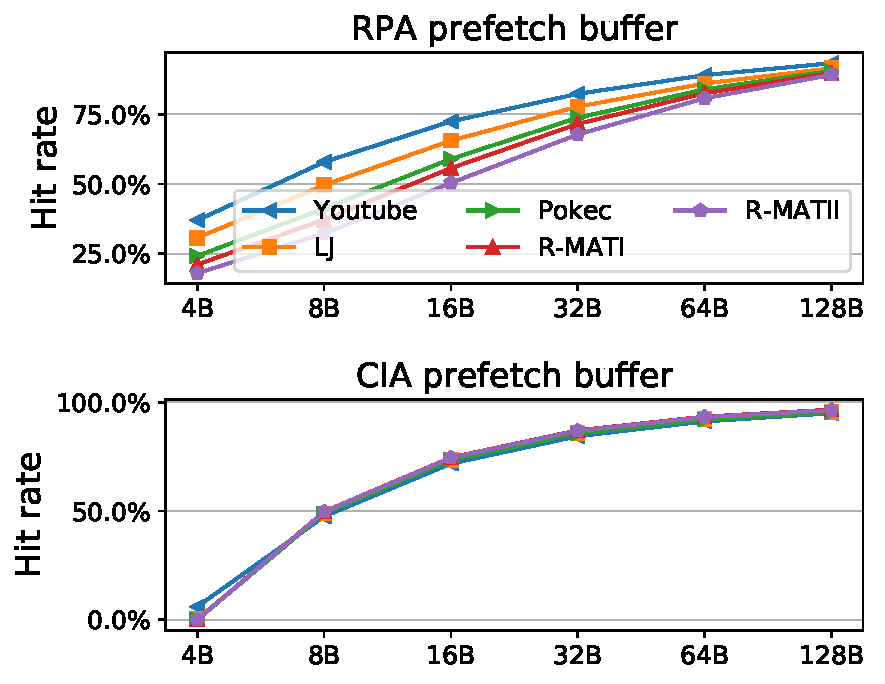
\includegraphics[width=0.95\linewidth]{prefetch-hit}}
    \caption{A small prefetch buffer can already achieve high hit rate.
    Particularly the prefetch buffer size influence on different graph 
    data set is similar.}
\label{fig:prefetch-hit}
\end{figure}

The FPGA resource consumption of the accelerator with optimized data path duplication 
strategies are presented in Table \ref{tab:duplicate-resource}. The accelerator 
with data path duplication incurs more logic resources including FF and LUT. 
Although the block RAM consumption doesn't increase too much, it remains the 
resource bottleneck mostly because of the large cache requirement.

\begin{table}
  \caption{FPGA resource consumption with data path duplication}
  \label{tab:duplicate-resource}
  %\setlength{\tabcolsep}{4pt} % Default value: 6pt
  %\renewcommand{\arraystretch}{1.5} % Default value: 1
    \centering
  \begin{tabular}{ccccccc}
    \toprule
      Config. & FF & \% & LUT & \% & RAMB18K & \% \\
    \midrule
      opt-DPD2  & 110150 & 12 & 185478 & 42 & 1893  & 64 \\
      opt-DPD4  & 194707 & 22 & 331870 & 70 & 809  & 84 \\
  \bottomrule
\end{tabular}
\end{table}

\subsection{Optimization evaluation}
As discussed in previous sub sections, we need hardware implementation 
to tune the pipelining depth while we can roughly decide the rest 
design parameters through software emulation. This ensures the HLS based 
BFS accelerator can be rapidly customized for each graph data set.

After tuning the design parameters, we evaluate the 
performance of the BFS accelerators with the optimization. 
Basically we start from the baseline design and 
add the optimizations including pipelining, hash redundancy removal, 
prefetching, caching and data path duplication in order. The performance improvement 
with these optimizations can be found in Figure \ref{fig:opt-performance}. 
In general, the performance of the BFS accelerator improves 
significantly when more optimization techniques are applied. Particularly,
pipelining and data path duplication enhance the performance most 
significantly. The performance improvement brought by the hash table based filtering 
seems to be trivial, but it actually boosts the performance by over 20\% on average. 
In addition, it also affects the cache efficiency as observed in Section \ref{sec:observation}
and is thus critical to the overall accelerator performance as well.

\begin{figure}
\center{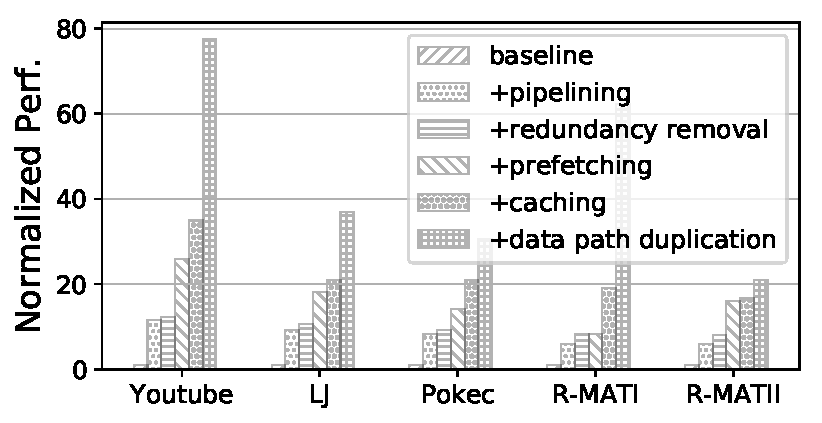
\includegraphics[width=0.95\linewidth]{opt-performance}}
    \caption{BFS accelerator optimization techqniue evaluation. The performance on 
    all the graphs improves when more optimizations including pipelining, 
    redundancy removal, prefetching, caching, and data path duplication are 
    gradually applied to the design.}
\label{fig:opt-performance}
\end{figure}

\section{Conclusions} \label{sec:conclusion}
Handcrafted HDL based BFS accelerators usually suffer high portability and maintenance cost 
as well as ease of use problem despite the relatively 
good performance. HLS based BFS accelerator can greatly alleviate these problems, but it is 
difficult to achieve satisfactory performance due to the inherent irregular memory access and 
complex nested loop structure. In this work, we stream the basic BFS algorithm and develop 
a series of HLS based optimizations such as redundancy removal, prefetching, caching and 
data path duplication. According to the experiments on 
a representative graph benchmark, the resulting HLS based BFS accelerator achieves up to 70X speedup 
compared to a baseline HLS design with best-effort HLS pragma optimization. When compared to the 
existing HDL based BFS accelerators on similar FPGA cards, the proposed HLS based BFS accelerator 
gets around 35\% of the MTEPS, but it preserves the nice software-like features including 
portability and ease of use and maintenance, and achieves higher per bandwidth MTEPS in some cases 
mostly because of the graph specific optimization techniques. 

